

We show the performance that can be expected from Multiple Oracle when using custom oracles on various important examples from the literature. In this section we present only the examples which we thought demonstrate interesting behaviors. In appendix \ref{appendix:do.results}, we follow with a more comprehensive evaluation of the algorithm using a generic master problem and oracles based on global optimization.

In some cases we show the progress of the convergence-criterion value \eqref{crit1} called ``instability'' over the course of $10$ iterations, and we also plot the Wasserstein distance \eqref{crit2} between mixed strategies in consecutive iterations. Each experiment was initialized with a randomly chosen feasible pure strategy. In games with polynomial utility functions, the best response oracles can employ both methods of the methods of global optimization described in Chapter \ref{ch:global}. In the rest of the games we use the spatial Branch and Bound approach as the best response oracle. From our experience, local solvers can work sufficiently well as oracles in some games.


\begin{example}[General Blotto]
    

The \emph{Double Oracle} algorithm converges unusually slowly (see Fig \ref{fig:ex.blotto.slow} for a game with 3 fronts) on the \emph{General Blotto} game valuing isolated fronts with $p=0.5$. Large gains are possible by winning a front by a small margin as the slope of the utility function around zero approaches infinity. After 40 iterations, the algorithm recovers the following $\epsilon$-NE with $\epsilon=0.03$:

\begin{figure}
\centering
\begin{tikzpicture}
\begin{groupplot}[
    group style={
        group size=2 by 1,
        horizontal sep=0.3cm
    },
    width=6cm,
    height=5cm,
    xlabel=Iteration,
    xmin=0,
    ymin=1e-6,
    xmax=41,
    ymode=log,
    legend style={
            at={(1.04,1.08)},
            anchor=south,
        legend columns=-1,
        column sep=1ex
    }
]

\pgfplotstableread{
0.41 0.41
0.29 0.29
0.29 0.35
0.24 0.1
0.22 0.51
0.18 0.068
0.11 0.25
0.12 0.17
0.091 0.15
0.1 0.11
0.094 0.11
0.18 0.085
0.14 0.11
0.1 0.13
0.12 0.076
0.069 0.11
0.074 0.078
0.071 0.091
0.043 0.049
0.061 0.045
0.043 0.046
0.046 0.046
0.045 0.062
0.045 0.031
0.054 0.038
0.024 0.053
0.043 0.048
0.06 0.054
0.054 0.058
0.047 0.039
0.033 0.039
0.038 0.028
0.032 0.025
0.038 0.02
0.03 0.029
0.029 0.023
0.019 0.026
0.027 0.025
0.029 0.023
0.021 0.032
}\exploitdata
\pgfplotstableread{
NaN NaN
1.2 1.2
0.6 0.87
0.44 0.41
0.71 0.81
0.65 0.57
0.42 0.22
0.33 0.21
0.21 0.18
0.18 0.15
0.14 0.17
0.17 0.17
0.16 0.27
0.14 0.21
0.12 0.15
0.14 0.14
0.14 0.17
0.11 0.11
0.1 0.098
0.16 0.11
0.17 0.11
0.13 0.074
0.12 0.062
0.11 0.054
0.048 0.073
0.1 0.078
0.082 0.083
0.091 0.097
0.071 0.079
0.096 0.06
0.083 0.069
0.089 0.092
0.06 0.07
0.034 0.083
0.063 0.064
0.06 0.087
0.062 0.09
0.044 0.047
0.056 0.046
0.074 0.049
}\wassersteindata

\pgfplotstablegetcolsof{\exploitdata}
\pgfmathtruncatemacro{\numcols}{\pgfplotsretval}

\nextgroupplot[ylabel=Exploitability]
\pgfplotsinvokeforeach{0,...,\numcols-1}{
    \addplot table[x expr=\coordindex+1, y index=#1] {\exploitdata};
}
\pgfplotsinvokeforeach{1,...,\numcols}{
    \addlegendentry{Player #1}
}

\nextgroupplot[ylabel=Wasserstein, ylabel near ticks, yticklabel pos=right]
\pgfplotsinvokeforeach{0,...,\numcols-1}{
    \addplot table[x expr=\coordindex+1, y index=#1] {\wassersteindata};
}

\end{groupplot}
\end{tikzpicture}
\caption{Slow convergence of a continuous but non-differentiable \emph{General Blotto} game valuing 3 isolated fronts with $p=0.5$. Both players can still profitably deviate by $0.02$ and $0.03$ utility units after 40 iterations. }
\label{fig:ex.blotto.slow}
\end{figure}

\begin{align*}
\mu_1^\star &\approx 0.003\delta_{ (0.15, 0.69, 0.16) } + 0.005\delta_{ (0.18, 0.16, 0.67) } + 0.006\delta_{ (0.57, 0.35, 0.08) } \\&+ 0.01\delta_{ (0.0, 0.5, 0.5) } + 0.011\delta_{ (0.45, 0.04, 0.51) } + 0.012\delta_{ (0.38, 0.11, 0.5) } \\&+ 0.018\delta_{ (0.09, 0.25, 0.66) } + 0.022\delta_{ (0.55, 0.01, 0.44) } + 0.026\delta_{ (0.06, 0.65, 0.29) } \\&+ 0.026\delta_{ (0.08, 0.52, 0.4) } + 0.029\delta_{ (0.49, 0.18, 0.32) } + 0.029\delta_{ (0.24, 0.16, 0.6) } \\&+ 0.032\delta_{ (0.44, 0.36, 0.2) } + 0.035\delta_{ (0.36, 0.0, 0.64) } + 0.039\delta_{ (0.04, 0.4, 0.55) } \\&+ 0.041\delta_{ (0.33, 0.12, 0.54) } + 0.041\delta_{ (0.28, 0.64, 0.08) } + 0.049\delta_{ (0.4, 0.02, 0.58) } \\&+ 0.051\delta_{ (0.2, 0.34, 0.46) } + 0.053\delta_{ (0.13, 0.55, 0.32) } + 0.061\delta_{ (0.26, 0.08, 0.66) } \\&+ 0.061\delta_{ (0.18, 0.58, 0.24) } + 0.069\delta_{ (0.0, 0.61, 0.39) } + 0.12\delta_{ (0.51, 0.45, 0.04) } \\&+ 0.151\delta_{ (0.64, 0.22, 0.14) },\\ 
\mu_2^\star &\approx 0.006\delta_{ (0.07, 0.66, 0.26) } + 0.009\delta_{ (0.0, 0.41, 0.59) } + 0.011\delta_{ (0.19, 0.59, 0.22) } \\&+ 0.012\delta_{ (0.54, 0.33, 0.13) } + 0.016\delta_{ (0.41, 0.14, 0.45) } + 0.02\delta_{ (0.0, 0.5, 0.5) } \\&+ 0.021\delta_{ (0.36, 0.4, 0.24) } + 0.023\delta_{ (0.44, 0.56, 0.0) } + 0.026\delta_{ (0.02, 0.61, 0.37) } \\&+ 0.028\delta_{ (0.14, 0.47, 0.39) } + 0.031\delta_{ (0.11, 0.26, 0.63) } + 0.033\delta_{ (0.37, 0.54, 0.09) } \\&+ 0.034\delta_{ (0.44, 0.51, 0.05) } + 0.037\delta_{ (0.5, 0.07, 0.43) } + 0.041\delta_{ (0.21, 0.32, 0.47) } \\&+ 0.045\delta_{ (0.05, 0.54, 0.41) } + 0.046\delta_{ (0.32, 0.06, 0.61) } + 0.055\delta_{ (0.47, 0.0, 0.53) } \\&+ 0.058\delta_{ (0.09, 0.61, 0.29) } + 0.06\delta_{ (0.28, 0.15, 0.57) } + 0.063\delta_{ (0.6, 0.03, 0.36) } \\&+ 0.064\delta_{ (0.24, 0.66, 0.1) } + 0.07\delta_{ (0.02, 0.32, 0.67) } + 0.087\delta_{ (0.56, 0.44, 0.01) } \\&+ 0.104\delta_{ (0.67, 0.17, 0.17) }.
\end{align*}


\begin{figure}
\centering
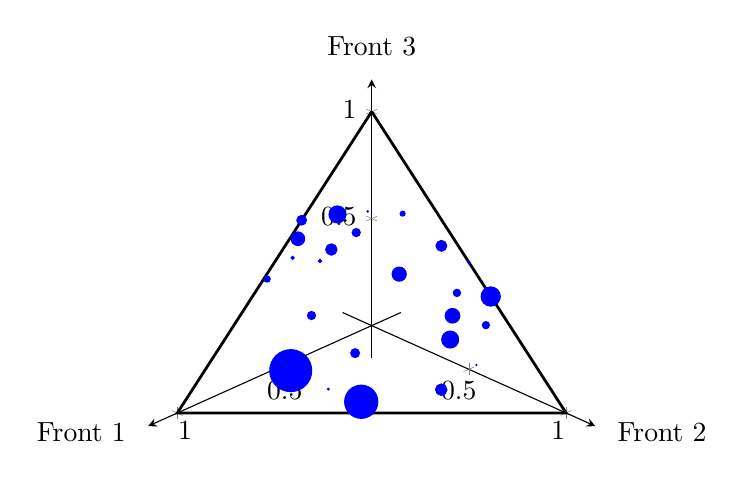
\begin{tikzpicture}
\begin{axis}[
    view={135}{30},
    xlabel={Front 1},
    ylabel={Front 2},
    zlabel={Front 3},
    xmin=0,
    xmax=1,
    ymin=0,
    ymax=1,
    zmin=0,
    zmax=1,
    width=8cm,
    height=8cm,
    axis lines=center,
    xlabel style={
        at={(ticklabel* cs:1.05)},
        anchor=east,
    },
    ylabel style={
        at={(ticklabel* cs:1.05)},
        anchor=west,
    },
    zlabel style={
        at={(ticklabel* cs:1.05)},
        anchor=south,
    },
    enlargelimits=0.15,
]
\addplot3[%
    scatter=true,
    only marks,
    mark=*,
    color=blue,
    point meta=explicit symbolic,
    scatter/@pre marker code/.style={/tikz/mark size=\pgfplotspointmeta*50},
    scatter/@post marker code/.style={}
] table[meta=w] {
x y z w
1.0 0.0 0.0 0.0
0.0 0.5 0.5 0.009654303207164589
0.25023023442966097 0.0 0.749769765570339 0.0
0.4932058353192057 0.18339681951996878 0.3233973451608256 0.029049980169382907
0.05650389511331322 0.8185970753584575 0.12489902952822926 0.0
0.41324231587781224 0.5867576841221878 0.0 0.0
0.6786405856065275 0.2903750381341887 0.03098437625928374 0.0
0.04349031055866048 0.4019373736382605 0.5545723158030791 0.038939095750905456
0.40076388878462343 0.021050456413010954 0.5781856548023656 0.04903090473416174
0.28243478105978426 0.6401915321648839 0.07737368677533185 0.04102671314930601
0.6648072334414368 0.0492306855836383 0.285962080974925 0.0
0.4814467233982045 0.5185532766017955 0.0 0.0
0.5468670648060134 0.00863406240441808 0.44449887278956846 0.022460565168244927
0.5862207793698717 0.39658897388822667 0.017190246741901616 0.0
0.17927649660562558 0.42246502397578034 0.39825847941859405 0.0
0.17632605612548735 0.5800034182869338 0.2436705255875789 0.06116312502553871
0.17595515345286916 0.15544262768706385 0.6686022188600669 0.004913497002613197
0.06062783145227446 0.6480035921955467 0.29136857635217883 0.02573772209026134
0.4434015332588057 0.3580189646073698 0.19857950213382447 0.0317522137806465
0.6505667816550538 0.1406871919800712 0.20874602636487505 0.0
0.0005920491605698741 0.6129137926298092 0.38649415820962096 0.0693668678563529
0.36046902825807403 0.0 0.639530971741926 0.03473597639610715
0.22308037099985156 0.27282562736959437 0.5040940016305541 0.0
0.13091929174218178 0.5465536126485865 0.3225270956092317 0.05273009731745313
0.3807376886206286 0.11485117054647198 0.5044111408328994 0.011743681147501262
0.5718755706169245 0.34901419767610814 0.0791102317069674 0.0059343257314523855
0.08158609957530605 0.5199658231548522 0.3984480772698417 0.02606561245934508
0.2523124234763152 0.5048769863677894 0.24281059015589534 0.0
0.2587178789380146 0.0824759880691166 0.6588061329928687 0.06115018279390709
0.31979246746766377 0.5397979595882282 0.14040957294410805 0.0
0.0897597760074555 0.2488346628453484 0.6614055611471962 0.017752319832239367
0.6033479577565064 0.29409578686799936 0.10255625537549427 0.0
0.4185724773649851 0.4447976227489905 0.13662989988602436 0.0
0.2405922803031214 0.160868318172387 0.5985394015244916 0.029275557559801872
0.1510666841314512 0.6895558742600341 0.1593774416085148 0.0034854601099706677
0.5082709727439931 0.4544398062393061 0.037289221016700735 0.1197678059454477
0.4460005375907148 0.03929476881514227 0.514704693594143 0.010953995589564676
0.3326427904764855 0.12496673516560852 0.542390474357906 0.04086140412689088
0.19889502688623395 0.34038407361247286 0.4607208995012932 0.0509852939350661
0.6379954308633884 0.2214620982069253 0.1405424709296862 0.15146329912067436
};
\addplot3[
    color=black,
    line width=1pt,
    mark=none,
] table {
x y z
0 0 1
0 1 0
1 0 0
0 0 1
};
\end{axis}
\end{tikzpicture}
\caption{The recovered strategy of Player 1 after 40 iterations drawn as points on a simplex with weight being indicated by their size. }
\label{fig:ex.blotto.slow.simplex}
\end{figure}
\end{example}

\begin{example}[Zero-sum polynomial game \cite{ParriloIEEE06}]\label{ex0}
    Consider a two-player zero-sum game with strategy sets $[-1,1]$ and a utility function of the first player
    \[
      u(x,y) = 2xy^2 - x^2 - y.
    \]

    As the generated subgames are all finite two-player zero-sum games, we can use linear programming to find their equilibria. The best response oracles were implemented using Lasserre's hierarchies.

    \begin{figure}
      \centering
      \label{figure0}
      
\includegraphics{do2.pdf}
      \caption{Convergence in Example \ref{ex0}. After 10 iterations, our method finds pure strategies $x \approx 0.4$ and $y \approx 0.63$, resulting in payoffs \((-0.47, 0.47)\). }
    \end{figure}
\end{example}

\begin{example}[General-sum polynomial game \cite{SteinOzdaglarParrilo08}]\label{ex1}
  The strategy set of each player is $[-1,1]$ and utility functions are
  \begin{align*}
    u_{1}(x,y) & = -3x^2y^2 - 2x^3 + 3y^3 + 2xy - x,\\
    u_{2}(x,y) &= 2x^2y^2 + x^2y - 4y^3 - x^2 + 4y.
  \end{align*}

  We computed equilibria in the general-sum matrix subgames using the multilinear program \ref{eq:sturmfels}. The best response oracles were implemented using Lasserre's hierarchies again.

  \begin{figure}
    \centering
    
\includegraphics{do3.pdf}
    \caption{Convergence in Example \ref{ex1}. Our method finds mixed strategies where $x\approx0.11$ with probability $44.19\%$ and $x\approx-1$ with probability $55.81\%$ and $y\approx0.72$ resulting in payoffs \((1.13, 1.81)\).}
  \end{figure}
\end{example}

\begin{example}[Torus game \cite{Chasnov20}]\label{ex2}
  Each strategy set is the unit circle $S^1 = [-\pi, \pi]$ and the utility functions are
  \begin{align*}
    u_{1}(\theta_1, \theta_2) &= \alpha_1 \cos(\theta_1 - \phi_1) - \cos(\theta_1 - \theta_2),\\
    u_{2}(\theta_1, \theta_2) &= \alpha_2 \cos(\theta_2 - \phi_2) - \cos(\theta_2 - \theta_1).
  \end{align*}
  parametrized by $\phi = (0, \pi/8)$ and $\alpha = (1, 1.5)$.

  We implemented the best response oracles using the spatial Branch and Bound method implemented by the \emph{Couenne} solver. We note that both the \emph{Gurobi} solver and \emph{SCIP} can also accept trigonometric functions as constraints. The general-sum master-problem was solved using the multilinear approach again.

  \begin{figure}
    \centering
    
\includegraphics[width=0.8\textwidth]{do1.pdf}
    \caption{Convergence in Example \ref{ex2}. We obtained pure strategies $\theta_1 \approx -1.06$, $\theta_2 \approx 1.01$ resulting in payoffs \((0.97, 1.71)\).}
  \end{figure}
\end{example}

\begin{example}[General Blotto \cite{Golman09}]\label{ex3}
  Each strategy set in this two-player zero-sum game is the standard $4$-dimensional simplex in $\R^5$ and the utility function of the first player is
  \[
    u(\textbf{x}, \textbf{y}) = \sum_{j=1}^5 f(x_j - y_j),
  \]
  where $f(x) = \sgn(x)\cdot x^2$.

  The master problem reduces to linear programming. We chose to implement the oracles using spatial Branch and Bound with symbolic reformulation (\cref{sec:sbab}) in \emph{Gurobi}. We modeled the $\sgn$ function using the following piecewise linear approximation:
  \[
    \sgn(x) \approx \begin{cases*}
      -1 & \text{if $x \le 0$}\\
      +1 & \text{otherwise}
    \end{cases*}.
  \]
  Since the multiplier $x^2$ will be zero, it is acceptable to ignore the behavior of this $\sgn$ approximation around zero.

  \begin{figure}
    \centering
    
\includegraphics[width=0.8\textwidth]{do6.pdf}
    \caption{Convergence in Example \ref{ex3}. We recovered pure strategies $\textbf{x} \approx (0, 0, 1, 0, 0)$ and $\textbf{y} \approx (1, 0, 0, 0, 0)$ resulting in payoffs \((0, 0)\). This is an~equilibrium computed by \textcite[Proposition 5]{Golman09}}
  \end{figure}
\end{example}


\begin{example}[Random polymatrix games]\label{exsep}
  Separable network games (polymatrix games) with finitely many strategies of each player can be solved in polynomial time \cite{Cai16} by linear programming. We use Algorithm \ref{alg:do} to compute equilibria of five-player polymatrix games defined by 20 by 20 matrices. Specifically, we generated a random matrix for each edge in the network and then transposed and subtracted the matrix of utility functions to make the game globally zero sum. We remark that zero-sum polymatrix games are payoff-equivalent to the general polymatrix games by \cite[Theorem 7]{Cai16}. In a test of 100 games, our algorithm found an $\eps$-equilibrium with $\eps = 0.01$ after $17.69$ iterations in a mean time of $0.29$ seconds.
\end{example}

\begin{example}[Three-player separable network game]\label{ex4}
  Further, we considered a continuous generalization of separable network games with strategy sets $[-1,1]$ and polynomial utility functions. This class of games was analyzed with the tools of polynomial optimization in \cite{KroVaVo}. There are 3 players. All pairs of players are involved in bilateral general-sum games and each player uses the same strategy across all such games. The pairwise utility functions are:
  \begin{equation*}
    \begin{aligned}
      u_{1, 2}(x_1,x_2) &= -2x_1x_2^2 + 5x_1x_2 - x_2\\
      u_{1, 3}(x_1,x_3) &= -2x_1^2 - 4x_1x_3 - 2x_3\\
      u_{2, 1}(x_2,x_1) &= 2x_1x_2^2 - 2x_1^2 - 5x_1x_2 + x_2\\
      u_{2, 3}(x_2,x_3) &= -2x_2x_3^2 - 2x_2^2 + 5x_2x_3\\
      u_{3, 1}(x_3,x_1) &= 4x_1^2 + 4x_1x_3 + 2x_3\\
      u_{3, 2}(x_3,x_2) &= 2x_2x_3^2 + 2x_2^2 - 5x_2x_3
    \end{aligned}
  \end{equation*}
  \begin{figure}
    \centering
    
\includegraphics{do7.pdf}
    \caption{Convergence in Example \ref{ex4}. Our method finds the mixed strategies where $x_1 \approx -0.06$, $x_2$ is $0.35$ with probability $0.708$ and $0.36$ with probability $0.292\%$, $x_3$ is $1.0$ with probability $0.7211$ and $-1.0$ with probability $0.2789$; with the corresponding payoffs \((-1.23, 0.26, 0.97)\).}
  \end{figure}
\end{example}
